\documentclass{article}
\usepackage{indentfirst}
\usepackage{lmodern}
\usepackage[utf8]{inputenc}
\usepackage[T1]{fontenc}
\usepackage[ngerman]{babel}
\usepackage{amssymb,amstext,amsmath}
\usepackage{graphicx}

%\renewcommand*{\size@chapter}{\Huge}

\usepackage{cite}
\usepackage{url}
 
\title{Die Elektromagnetische Induktion}
\author{Alexander Heinisch, Dominik Wille}
\begin{document}
\maketitle
\vspace{13cm}
\noindent
%\begin{center}
\begin{tabular}{l l}
Tutor & Matthias Bernien  \\
Durchführung & 17. April 2013 \\

E-Mail Dominik & dominik.wille@fu-berlin.de \\
E-Mail Alexander & matthias.heinisch@gmx.de \\
\end{tabular}
%\end{center}

\newpage
\tableofcontents
\newpage

\section{Einleitung}

In diesem Protokoll werden Experimente zur elektromagnetischen Induktion ausgewertet und diskutiert, dabei geht es vor allem darum, die Vorhersagen aus der Elektrodynamik bzw. den {\sc Maxwellschen Gleichungen} zu überprüfen.
 
\subsection{Die Maxwellschen Gleichungen}

Die Maxwellschen Gleichungen bilden einen Satz von Formeln, aus denen eine mathematische Beschreibung elektromagnetscher Probleme ableitbar ist.\\ \\
Die Gleichungen haben folgende Form:

\begin{equation}\label{maxwell1}
\operatorname{div} \vec{E} = \frac{\rho(\vec{r})}{\varepsilon_0}
\end{equation}
\begin{equation}\label{maxwell2}
\operatorname{div} \vec{B} = 0
\end{equation}
\begin{equation}\label{maxwell3}
\operatorname{rot} \vec{E} + \frac{\partial \vec{B}}{\partial t}= 0
\end{equation}
\begin{equation}\label{maxwell4}
\operatorname{rot} \vec{B} - \mu_0 \varepsilon_0 \frac{\partial \vec{E}}{\partial t} = 0
\end{equation}

\noindent
Die ausführliche Diskussion der Gleichungen soll nicht Teil dieses Protokolls sein. Da sich aber die theoretische Betrachtung auf diese Gleichungen stützt und diese im Allgemeinen von elematarer Wichtigkeit für die Elektrodynamik sind, seien sie dennoch erwähnt.

\section*{Aufgabenstellung}
\subsection*{Aufgabe 1}
Untersuchung der Induktionsspannung in Abhängigkeit von der Zeit an einer Probespule (Induktionsspule) innerhalb einer Magnetspule (Feldspule) beim Anlegen einer Rechteckspannung an die Feldspule. Berechnung der induzierten Spannung \(U_0\) für \(t=0\) und des Selbsinduktionskoeffizienten \(L\) der Feldspule. Vergleich der Ergebnisse mit den theoretischen Erwartungen.
\subsection*{Aufgabe 2}
Messung der Induktionsspannung (Effektivwert) an der Induktionsspule bei einem sinusförmigen Wechselstrom durch die Feldspule in Abhängigkeit von der Frequenz des Feldstroms. Qualitativer und quantitativer Vergleich des Ergebnisses mit der theoretischen Erwartung.
\subsection*{Aufgabe 3}
Messung der Induktionsspannung bei einem Wechselstrom durch die Feldspule in Abhängigkeit von der Orientierung der Induktionsspule bei einer Frequenz von 100 Hz. Zusätzliche Messung bei einer Frequenz von 1 kHz bei der Winkeleinstellung \(0^\circ \). Qualitativer und quantitativer Vergleich der Ergebnisse mit den theoretischen Erwartungen.

\section{Theoretische Vorbetrachtung}
\subsection{Induktionsspannung}
Aus \eqref{maxwell3} folgt die integrale Schreibweise, wobei \(A\) die vom Magnetfeld durchflossene Fläche bezeichnet
\begin{equation*}
\int_{A}\operatorname{rot} \vec{E} \cdot d\vec{A} =  
\int_{A} -\frac{\partial \vec{B}}{\partial t} \cdot d\vec{A}
\end{equation*}
Die Ableitung nach der Zeit kann vor das Integral gezogen werden, da in diesem Fall die Fläche nicht von der Zeit abhängt. Durch Anwendung des {\sc Stokesschen Integralsatzes} auf die linke Seite der Gleichung formt sich die Gleichung folgendermaßen um
\begin{equation*}
\int_{\partial A}\vec{E} \cdot d\vec{s} =  
-\frac{d}{dt} \int_{A} \vec{B} \cdot d\vec{A}
\end{equation*}
Bei der linken Seite handelt es sich nach Definition um eine {\sc elektrische Spannung}. Da diese durch die Änderungen des Magnetfelds induziert wird, nennt man sie Induktionsspannung. Der Zusammenhang wurde erstmals von Michael Faraday beschrieben und wird daher auch {\sc Faraday'sches Induktionsgesetz} genannt.

\begin{equation}\label{faraday}
U_{ind} =  
-\frac{d}{dt} \int_{A} \vec{B}(\vec{r}) \cdot d\vec{A}
\end{equation}

\subsection{Das Magnetfeld einer Spule}
Um eine theoretische Betrachtung der Problemstellung zu machen, ist es vorteilhaft einige Näherungen einzugehen. Im Rahmen des Protokolls soll das Magnetfeld auf der zentralen Achse in der Spule bestimmt werden. Um dies zu bestimmen, soll die Dicke der Windungen vernachlässigbar klein sein. Außerdem wird im folgenden davon ausgegangen, dass der Strom der Spule perfekt kreisförmig und nicht spiralförmig fließt. Desweiteren soll er absolut gleichverteilt über eine Zylinderoberfläche fließen. Mit diesen Näherungen kann die Stromdichteverteilung \( \vec{j}(\vec{r}) \) einer Spule der Länge \(l\) und dem Radius \(R\) in Zylinderkoordinaten beschrieben werden als

\begin{equation}
\vec{j}(\vec{r}) = \frac{IN}{l}\delta(\rho - R) \theta(z+\frac{l}{2}) \theta(z-\frac{l}{2}) \hat{e}_\varphi
\end{equation}

Mit dem {\sc Biot-Savart-Gesetz}, das aus den {\sc Maxwell-Gleichungen} ableitbar ist aber hier als gegeben benutzt wird erhält man


\begin{align}
\tag{Biot-Savart-Gesetz}
\vec{B}(\vec{r}) &=           \frac{\mu_0}{4\pi}\int_V \vec{j}(\vec{r}') \times
\frac{\vec{r}-\vec{r}'}{|\vec{r}-\vec{r}'|^3} \, d^3r'
\\
\vec{B}(\vec{r}) &= \frac{\mu_0}{4\pi}\int_{-\infty}^\infty \int_0^{2\pi} \int_{-\infty}^\infty
\vec{j}(\vec{r}') \times \frac{\vec{r}-\vec{r}'}{|\vec{r}-\vec{r}'|^3} 
\, r' \, dr' \, d\varphi' \, dz'
\notag
\\
&= \frac{\mu_0}{4\pi}\int_{-\infty}^\infty \int_0^{2\pi} \int_{-\infty}^\infty
\frac{IN}{l}\delta(\rho - R) \theta(z+\frac{l}{2}) \theta(z-\frac{l}{2}) \hat{e}_\varphi' \times
\frac{\vec{r}-\vec{r}'}{|\vec{r}-\vec{r}'|^3}  \, r' \, dr' \, d\varphi' \, dz'
\notag
\\
&= \frac{\mu_0}{4\pi}\int_{-l/2}^{l/2} \int_0^{2\pi} \frac{IN}{l} \hat{e}_\varphi'
\times \frac{z\hat{e}_z-R\hat{e}_r'-z'\hat{e}_z'}{|z\hat{e}_z-R\hat{e}_r'-z'\hat{e}_z'|^3} \, R \, d\varphi' \, dz'
\notag
\\
&= \frac{\mu_0}{4\pi}\int_{-l/2}^{l/2} \int_0^{2\pi} \frac{IN}{l}
\frac{(z-z')\hat{e}_r'+R\hat{e}_z'}{((z-z')^2+R^2)^{3/2}} \, R \, d\varphi' \, dz'
\notag
\\
 &= \frac{\mu_0}{2}\int_{-l/2}^{l/2} \frac{IN}{l}
\frac{R^2\hat{e}_z'}{((z-z')^2+R^2)^{3/2}} \, dz'
\notag
\\
\notag
\\
&z-z' = R \tan (\alpha) \Rightarrow dz' = -R(1 + \tan^2(\alpha)) d \alpha
\tag{Substitution}
\\
\notag
\\
\vec{B}(\vec{r}) &= \frac{\mu_0}{2}\int -\frac{IN}{l}
\frac{(1+\tan^2(\alpha))}{(1+\tan^2(\alpha))^{3/2}}\hat{e}_z \, d \alpha
\notag
\\
\notag
\\
&(1 + \tan^2(\alpha)) = \frac{1}{\cos^2(\alpha)}
\notag
\\
\notag
\\
\vec{B}(\vec{r}) &= -\frac{\mu_0 I N}{2 l}\int
\cos (\alpha) \, d \alpha
=  -\frac{\mu_0 I N}{2 l} \sin (\alpha)
\notag
\\
\notag
\\
& \sin (\alpha) = \frac{\tan (\alpha)}{\sqrt{1+\tan^2 (\alpha)}}
= \frac{\frac{z-z'}{R}}{\sqrt{1+(\frac{z-z'}{R})^2}} \; ; \, a =  - z -\frac{l}{2}
\notag
\\
\notag
\\
\vec{B}(\vec{r}) &= -\frac{\mu_0 I N}{2 l} \left(\frac{z+l/2}{\sqrt{R^2+(z+l/2)^2}}-\frac{z-l/2}
{\sqrt{R^2+(z-l/2)^2}}\right)
\notag
\\
\vec{B}(\vec{r}) &= \frac{\mu_0 I N}{2 l} 
\left(\frac{a}{\sqrt{R^2+a^2}}+\frac{l-a}{\sqrt{R^2+(l-a)^2}}\right)
\label{magnetfeld}
\end{align}
\newpage

Um mit dieser Lösung für das Magnetfeld zu rechnen, ist es praktisch das Magnetfeld im Innern der Spule als konstant anzunehmen. Um einen  vernünftigen Wert für das Magnetfeld zu erhalten ist über die gesamte Länge der Spule zu mitteln. Es sei

\begin{equation}
F(a)= \frac{1}{2} \left(\frac{a}{\sqrt{R^2+a^2}}+\frac{l-a}{\sqrt{R^2+(l-a)^2}}\right)
\notag
\end{equation}

\noindent
ein Korrekturfaktor, der gemittelt über die Gesamtlänge bezeichnet wird als

\begin{equation}
\bar{F}(l) = \frac{1}{l}\int_0^l F(a) \, da = \frac{1}{l} \left( \sqrt{R^2+l^2}-R \right)
\notag
\end{equation}

\noindent
Dadurch vereinfacht sich das Magnetfeld zu

\begin{equation}
\bar{B}(l) = \mu_0 \frac{ N I}{l} \bar{F}(l)
\label{magnetfeld_const}
\end{equation}
\subsection{Selbstinduktion}
Da sich beim aus- oder einschalten ein Magnetfeld bildet, führt dies zu einer Wechselwirkung der Spule mit sich selbst. Dieses Verhalten bezeichnet man als Selbstinduktion.
Für eine Spule mit \(N\) Windungen wird \eqref{faraday} zu

\begin{equation}
U_{ind} = - N \frac{d}{dt} \int_{A} \vec{B}(\vec{r}) \cdot d\vec{A}
\notag
\end{equation}
\noindent
Da \(\vec{B}\) als konstant in der Spule anngenommen wird, wird daraus

\begin{equation}
U_{ind} = - N \cdot A \cdot \frac{d \bar{B}}{dt} 
\label{U_ind_allg}
\end{equation}
\noindent
Durch einsetzetn von \eqref{magnetfeld} wird das zu

\begin{equation}
U_{ind} = - \mu_0 \cdot N^2 \cdot \frac{A}{l} \cdot  \bar{F}(l) \cdot \frac{dI(t)}{dt}
\notag
\end{equation}
\noindent
Man bezeichnet die Proportionalitätskonste zwischen \(U_{ind}\) und \(I\) als Selbstinduktionskoeffitient

\begin{equation}
L = \mu_0 \cdot N^2 \cdot \frac{A}{l} \cdot  \bar{F}(l)
\label{selbstinduktionkoeff}
\end{equation}
\noindent
Für \(U_{ind}\) gilt somit
\begin{equation}
U_{ind} = -L \cdot \frac{dI(t)}{dt}
\label{selbstinduktion}
\end{equation}

\newpage

\subsection{Induktion durch Ein- und Ausschaltvorgänge}
Beim Ein- und Ausschalten einer Spule entfällt sowohl bei der Spule als auch bei der Stromquelle ein Teil der Leistung, da es sich nicht um perfekte Bauelemente handelt. Rechnerisch soll der Innenwiederstand der Stromquelle als \(R_I\) und der ohmsche Widerstand der Spule als \(R_L\) bezeichnet werden. Da nach der {\sc Lenz'schen Regel} die Wirkung immer entgegen der Ursache wirkt  muss die Induktionsspannung der Eingangsspannung entgegenwirken. Somit gilt

\begin{equation}
U_{Ges} = I(R_L+R_I) - U_{ind}
\notag
\end{equation}
\noindent
Durch einsetzen von \eqref{selbstinduktion} wird das zu

\begin{equation}
U_{Ges} = I(R_L+R_I) + L \cdot \frac{dI}{dt}
\label{einaus_dgl}
\end{equation}
\noindent
es handelt sich um eine lineare inhomogene Differentialgleichung 1. Ordnung.
Die Lösung ist somit die Summe aus der Lösung der zugehörigen homogenen Differentialgleichung und einer speziellen Lösung. Die dazugehörige homogene Differentialgelichung lautet

\begin{equation}
0 = I(R_L+R_I) + L \cdot \frac{dI}{dt}
\notag
\end{equation}
\noindent
und hat die Lösung
\begin{equation}
I(t) = A \cdot e^{-\frac{1}{L}(R_L+R_I)t}
\notag
\end{equation}
\noindent
Eine spezielle Lösung der Gleichung ist

\begin{equation}
I(t) = \frac{U_{G}}{R_L+R_I}
\notag
\end{equation}
\noindent
Die allgemeine Lösung von \eqref{einaus_dgl} ist somit
\begin{equation}
I(t) = A \cdot e^{-\frac{1}{L}(R_L+R_I)t} + \frac{U_{G}}{R_L+R_I}
\label{einaus_dgl_lsg}
\end{equation}
\noindent
Es soll ein Umschaltvorgang von \(-U_{Ges}\) zu \(+U_{Ges}\) betrachtet werden.
Da zum Zeitpunkt \(t=0\) nur die ohm'schen Widerstände wirken gilt
\begin{equation}
I(t=0) = -\frac{U_{G}}{R_L+R_I}
\notag
\end{equation}
\noindent
\eqref{einaus_dgl_lsg} wird daher zu
\begin{equation}
I(t) = \frac{U_{G}}{R_L+R_I} \cdot \left(1-2 \cdot e^{-\frac{1}{L}(R_L+R_I)t} \right)
\notag
\end{equation}
\noindent
Damit gilt für die Spannung nach  \eqref{selbstinduktion}
\begin{equation}
U(t) = -2 U_{G}\cdot e^{-\frac{1}{L}(R_L+R_I)t}
\notag
\end{equation}

\subsection{Induktion durch Wechselfelder}
Bei normalem sinusförmigen Wechselstrom kann der Stromverlauf beschrieben werden durch
\begin{equation}
I(t) = I_0 \sin(\omega t + \varphi_0)
\notag
\end{equation}
\noindent
und für die induzierte Spannung nach  \eqref{selbstinduktion}
\begin{equation}
U(t) = U_0 \cdot \cos(\omega t + \varphi_0)\, ; \, U_0 = I_0 \omega
\notag
\end{equation}
\noindent
Der Effektivwert ist

\begin{align}
U_{eff} &= \sqrt{\frac{1}{T} \int_o^T U_0^2 \cos^2(\omega t + \varphi_0) \, dt}
\notag
\\
U_{eff} &= \sqrt{\frac{U_0^2}{2 \omega T} 
\left( \omega T + \sin(\varphi_0) \cos(\varphi_0) - 
\sin(2\pi + \varphi_0) \cos(2\pi + \varphi_0) \right)}
\notag
\\
U_{eff} &= \frac{U_0}{\sqrt{2}}
\label{U_eff}
\end{align}

\section{Aufgabe 1}

\subsection{Aufbau}
Der Funktionsgenerator wurde mit Verbindungskablen an die Feldspule mit \(n=1000\) Windungen angeschlossen und zusätzlich mit dem 1. Kanal des Oszilloskops verbunden. Die Frequenz wurde auf \(f=102,7\,Hz\) eingestellt. Die Induktionsspule wurde an den zweiten Kanal angeschlossen. Nachdem eine gute Einstellung für das Oszilloskop gefunden war, wurden die Messbereiche folgendermaßen festgelegt:
\begin{center}
\begin{tabular}{l l} 
Messgröße & Messbereich \\
  \(U_{Feld}\) & 2V \\ 
  \(U_{Ind}\) & 1V \\ 
  \(U_0\) & 2V \\ 
  \(U_\infty \) & 0,1V \\ 
 \end{tabular}
\end{center}

\subsection{Fehlerabschätzung}

Da die Messwerte nur durch Ablesen vom Oszilloskop ermittelt wurden ist der mit Abstand größte Fehler der Ablesefehler, da wir nur mit einer geschätzten genauigkeit von \( 1mm \) den Spannungsverlauf ablesen konnten.

Die Spannung wurde immer an waagerechten Gitterlinien abgelesen, daher ist \(\Delta t \ll \Delta U \). Um von dem Ablesefehler auf den Fehler der Spannung zu kommen, muss einfach nur mit der Skaleneinheit multipliziert werden, daher gilt für die \(2V\)-Skala \(\Delta U = 0,2V\) und für die \(1V\)-Skala \(\Delta U = 0,1V\). Da \(U_0\) durch die stark fallende Kurve schwer ablesbar war sei der Fehler in diesem Fall \(\Delta s = 3mm \Rightarrow \Delta U_0 = 0,6V \).

\subsection{Gegebenes}

Um die Induktivität der Feldspule aus deren Geometrie auszurechnen, setzt man nun in \eqref{selbstinduktionkoeff} ein

\begin{align}
L &= \mu_0 \cdot N^2 \cdot \frac{A}{l^2} \cdot \left( \sqrt{R^2+l^2}-R \right)
\notag
\\
 &= \mu_0 \cdot N^2 \cdot \frac{A}{l^2} \cdot \left( \sqrt{\frac{A}{\pi}+l^2}-\sqrt{\frac{A}{\pi}} \right)
\notag
\\
&= 11,44 \, mH
\end{align}
Der Fehler soll hier vereinfachend nur für die rechte Seite berechnet werden, da die konkreten Ausdrücke zu lang wären. Es handelt sich somit nur um eine grobe Abschätzung 
\begin{align}
\Delta L &= \sqrt{
	\left(\frac{\partial L}{\partial A} \Delta A \right)^2 +
	\left(\frac{\partial L}{\partial l} \Delta l \right)^2 }
\notag
\\
&= L \cdot \sqrt{
	\left(\frac{\Delta A}{A} \right)^2 +
	\left(\frac{-2 \Delta l }{ l}  \right)^2 }
\notag
\\
&= 0,24 \, mH
\notag
\end{align}
gemessen, gegeben oder errechnet wurden folgende Werte

\begin{center}
\begin{tabular}{r c c c}
 & & Feldspule & Induktionsspule \\
gegeben & \(N\) & \(1000\) & \(500\) \\
gegeben & \(A\) & \(19,73\,cm^2\) & \(15,95\,cm^2\) \\
gegeben & \(l\) & \((190 \pm 1)\, mm\) & \((190 \pm 1)\, mm\) \\
gemessen & \(R_L\) & \((7,1 \pm 0,1)\, \Omega \) & \((3,1 \pm 0,1)\, \Omega \) \\
gemessen & \(L\) & \((10,89 \pm 0,03)\, mH \) & \((2,268 \pm 0,008)\, mH \) \\
errechnet & \(L\) & \((11,44 \pm 0,24)\, mH \) & nicht  benötigt \\

\end{tabular}
\end{center}

\subsection{Beobachtung}

Qualitativ ist die Spannungskurve auf dem Oszilloskop für die Feldspule und für die Induktionsspule eine abfallende Kurve, die für die Induktionsspule gegen \(0V\) und für die Feldspule gegen einen Grenzwert \( U_\infty \) geht. 

\subsection{Messwerte und Graphen}
\begin{center}

\begin{tabular}{l l l l l}
Zeit [\(\mu s\)] & \(U_{Abs}[V]\) & \(U_{rel}\)[V] & \(ln(U_{rel})[V]\) & \(\Delta\ U_{rel}[V]\) \\
\(0\) & \(7\)	& \(6.56\) &	\(1.8810\) & 0.0625\\
\(50\) & \(5.5\) &	\(5.06\) &	\(1.63\) &  0.08 \\
\(100\) &	\(4.4\) &	\(3.96\) &	\(1.38\) &  \(0.11\)\\
\(150\) &	\(3.6\) &	\(3.16\) &	\(1.16\) & \(0.12\)\\
\(200\) &	\(2.8\) &	\(2.36\) &	\(0.86\) & \(0.19\)\\
\(250\) &	\(2\) &	\(1.56\) &	\(0.45\) & \(0.25\) \\
\(300\) &	\(1.7\) &	\(1.26\) &	\(0.24\) & \(0.29\) \\
\(350\) &	\(1.3\) &	\(0.86\) &	\(-0.15\) & \(0.45\) \\
\(400\) &	\(1\) &	\(0.56\) &	\(-0.58\) & \(0.67\) \\
\(450\) &	\(0.8\) &	\(0.36\) &	\(-1.0\) & \(1.00\) \\
\(500\) &	\(0.6\) &	\(0.16\) &	\(-1.8\) & \(2.00\) \\
\end{tabular}\\

Messung der Feldspulenspannung in Abhängigkeit von der Zeit\\
\vspace{1cm}
\begin{tabular}{l l l l}
Zeit [\(\mu s\)] & \(U_{Ind}[V]\) & \(ln(U_{Ind})[V]\) & \(\Delta\ U_{Ind}[V]\) \\
\(0\) &	\(3.2\) &	\(1.1632\) &	\(0.0625\)\\
\(50\) &	\(2.5\) &	\(0.92\) &	\(0.08\)\\
\(100\) &	\(1.9\) &	\(0.65\) &	\(0.11\)\\
\(150\) &	\(1.7\) &	\(0.53\) &	\(0.12\)\\
\(200\) &	\(1.0\) &5	\(0.049\) &	\(0.19\)\\
\(250\) &	\(0.8\) &	\(-0.23\) &	\(0.25\)\\
\(350\) &	\(0.45\) &	\(-0.80\) &	\(0.45\)\\
\(400\) &	\(0.3\) &	\(-1.21\) &	\(0.67\)\\
\(450\) &	\(0.2\) &	\(-1.61\) &	\(1.00\)\\
\(500\) &	\(0.1\) &	\(-2.31\) &	\(2.00\)\\

\end{tabular}\\
Messung der Induktionsspulenspannung in Abhängigkeit von der Zeit\\
\end{center}
\newpage
\begin{center}

  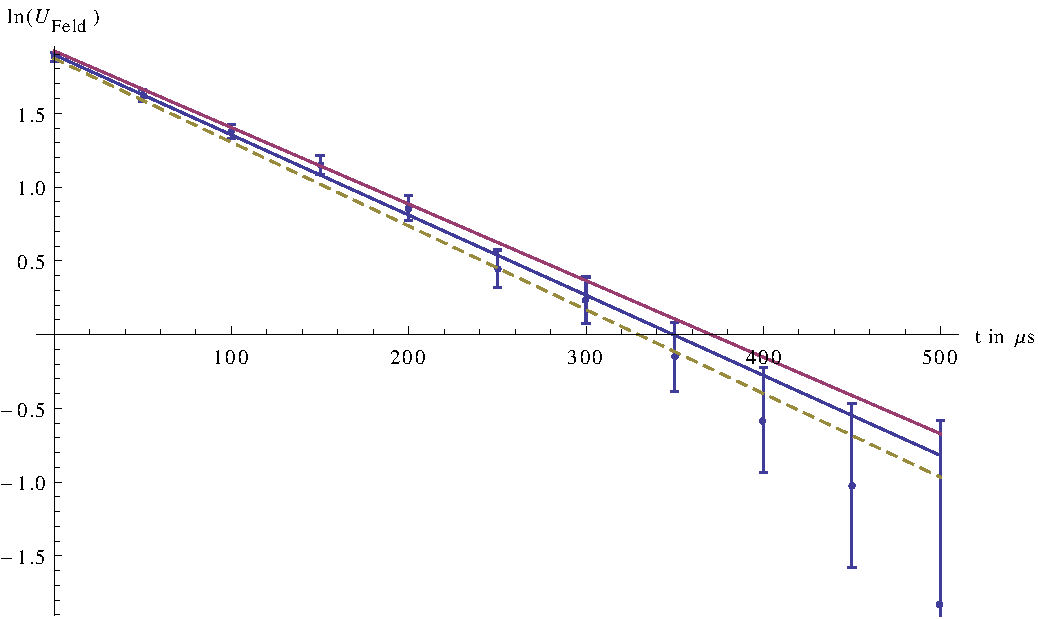
\includegraphics[width=11cm]{graph1}
	Spannungsverlauf bei der Feldspule

	\centering
  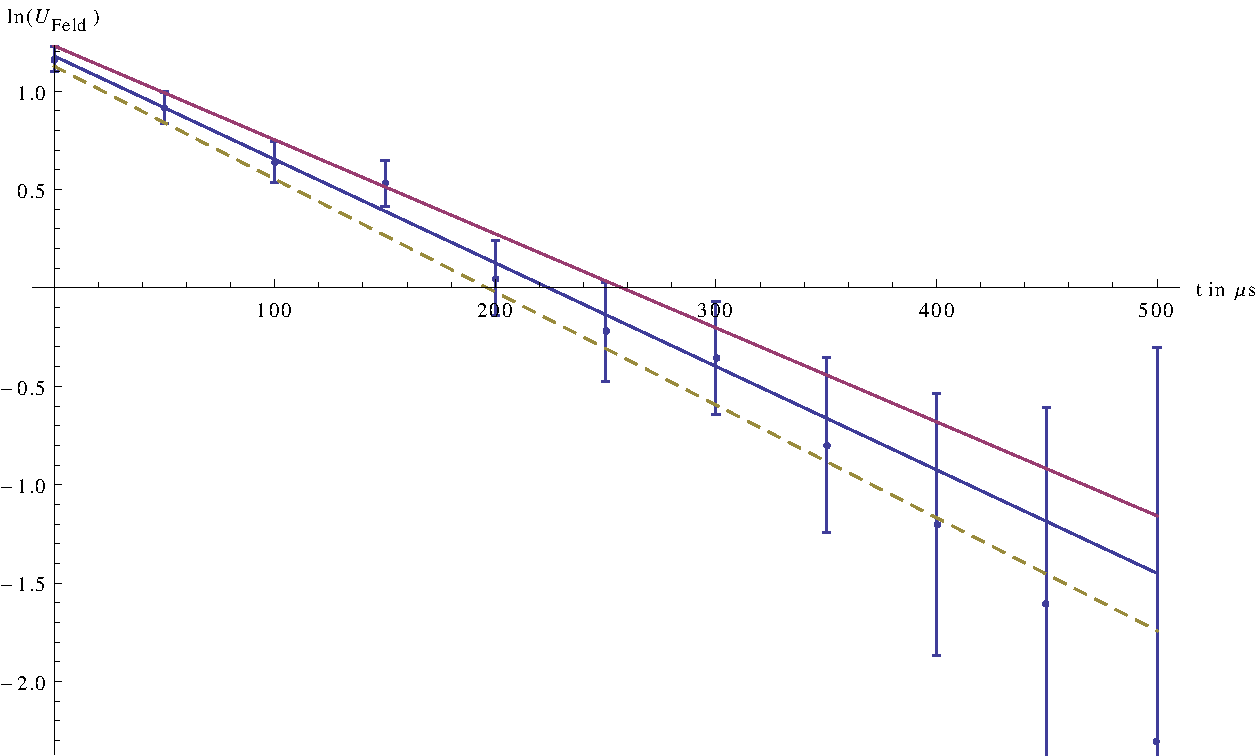
\includegraphics[width=11cm]{graph2}
	Spannungsverlauf bei der Induktionsspule
\end{center}

\noindent
Die Steigungen \(b\) und die Ordinatenabschnitte \(a\) wurde mittels linearer Regression bestimmt zu

\begin{center}
\begin{tabular}{c c c c c} 
  \(b_{Feld}\) & = & \(-5400\) & \(\pm \) & \(240 \) \\ 
  \(a_{Feld}\) & = & \(1,896\) & \(\pm \) & \(0,025 \) \\ 
  \(b_{Ind}\) & = & \(-5260\) & \(\pm \) & \(480 \) \\ 
  \(a_{Ind}\) & = & \(1,179\) & \(\pm \) & \(0,052 \) \\ 

 \end{tabular}
\end{center}

\subsection{Auswertung}

Um die vorhergesagte Messkurve überprüfen zu können, wurde die Spannung logarithmiert bzw. linearisiert. Für den Fehler \(ln(U)\) gilt

\begin{align}
\Delta ln(U) = \sqrt{\left(\frac{\partial ln(U)}{\partial U} \Delta U \right)^2} = \frac{\Delta U}{U}
\notag
\end{align}
\noindent
Wir betrachten \(-U(t)\), daher gilt

\begin{equation}
\label{U(t)}
ln(U) = ln(2U_G) - \frac{R_L+R_i}{L} t
\end{equation}


\noindent
daraus wird ersichtlich, dass



\begin{equation}
b = - \frac{R_L + R_I}{L}
\notag
\end{equation}
und
\begin{equation}
a = ln(2 U_G)
\notag
\end{equation}

\subsubsection{Feldspule}
Um daraus die Induktivität \(L_{Feld}\) zu bestimmen, ist noch ein bisschen Vorarbeit zu leisten.

In hinreichend langer Zeit wirkt nur noch der ohmsche Widerstand und es gilt
\begin{equation}
I_\infty = \frac{U_\infty}{R_L}
\notag
\end{equation}
\noindent
Aus \eqref{einaus_dgl_lsg} folgt für 
\begin{equation}
I_\infty = \frac{U_G}{R_L+R_I}
\notag
\end{equation}
Durch gleichsetzten folgt
\begin{align}
R_I &= \frac{R_L \left( U_G - U_\infty \right)}{U_\infty} = 
R_L \left(\frac{U_G}{U_\infty} - 1 \right) = 46,6 \, \Omega
\label{R_I}
\\
\Delta R_I &= \frac{\Delta U_G}{U_\infty} \cdot R_L = 1,3 \, \Omega
\end{align}

\noindent
aus \eqref{U(t)} folgt 

\begin{align}
a_{Feld} &= ln(2U_G)
\notag
\\
U_G &= \frac{1}{2} \cdot e^{a_{Feld}} = 3,329 \, V
\notag
\\
\Delta U_G &= \frac{1}{2} \cdot e^{a_{Feld}} \cdot \Delta a_{Feld} = 0,083 \, V
\notag
\end{align}
\noindent
und außerdem

\begin{align}
b_{Feld} &= - \frac{R_L + R_I}{L_{Feld}}
\notag
\\
L_{Feld} &= - \frac{1}{b_{Feld}} \cdot \left( R_L + R_I \right)
\notag
\end{align}
Mit \eqref{R_I} wird daraus 
\begin{align}
L &= - \frac{R_L}{b_{Feld}} \cdot \frac{U_G}{U_\infty} = 9,95 \, mH
\notag
\\
\Delta L &= 
L \cdot \sqrt{\left( \frac{\Delta b_{Feld}}{b_{Feld}} \right)^2 + \left( \frac{\Delta U_G}{U_G} \right)^2}
= 0,51 \, mH
\notag
\end{align}

\subsubsection{Induktionsspule}

Nach \eqref{U_ind_allg} gilt für jede Spule mit Querschnittsfläche \(A\), wenn das Magnetfeld als Ortsunabhängig angenommen wird

\begin{equation}
U_{ind} = -N \cdot A \cdot \frac{\partial B}{\partial t}
\label{U_induktionsspule}
\end{equation}
Außerdem folgt aus \eqref{magnetfeld_const} mit \eqref{selbstinduktionkoeff} 

\begin{equation}
B(t) = \frac{L_{Feld}}{n_{Feld} \cdot A_{Feld}} \cdot I(t)
\label{B_induktionsspule}
\end{equation}
Mit \eqref{einaus_dgl_lsg} folgt für \( U_{Ind} \)

\begin{equation}
U_{Ind} = \frac{n_{Ind} \cdot A_{Ind}}{n_{Feld} \cdot A_{Feld}}  \cdot \left(-2U_G \right) \cdot 
e^{-\frac{1}{L_{Feld}} \left( R_L + R_I \right)t}
\notag
\end{equation}
Um mit den Koeffizienten \(a_{Ind}\) und \(b_{Ind}\) zu vergleichen logarithmiert man \(-U_{Ind} \) zu
\begin{equation}
ln(U_{Ind}) = ln \left( \frac{n_{Ind} \cdot A_{Ind}}{n_{Feld} \cdot A_{Feld}}  \cdot 2U_G \right) \cdot \left( -\frac{1}{L_{Feld}} \left( R_L + R_I \right)t \right)
\notag
\end{equation}
Daraus wird ersichtlich, dass \(b_{Feld} = b_{Ind}\). Sei außerdem
\begin{align}
C &=  \frac{n_{Ind} \cdot A_{Ind}}{n_{Feld} \cdot A_{Feld}}  \cdot 2U_G = 2,69 \, V
\notag
\\
\Delta C &= C \cdot \frac{\Delta U_G}{U_G} = 0,07 \, V
\notag
\end{align}
Um \(C = e^{a_{Ind}} \)Vergleichen zu können rechnet man noch
\begin{align}
e^{a_{Ind}} &= 3,2 \, V
\notag
\\
\Delta e^{a_{Ind}} &= e^{a_{Ind}} \cdot \Delta a = 0,2 \, V
\notag
\end{align}

\subsection{Fazit und Vergleich}
Insgesamt waren alle Messungen verträglich mit den theoretischen Vorhersagen bzw. den gegebenen und gemessenen Werten im Einzelnen bedeutet das
\vspace{0.2cm}
\begin{center}
\begin{tabular}{r c c} 
  Messgröße & Messwert & Angabe/Theorie \\
  \(U_0\) & \( (7,6 \pm 0,4)\, V \) & \( (6,7 \pm 0,2)\, V \) \\
  \(L_{Feld}\) & \( (10,0 \pm 0,6)\, mH \) & \( (10,89 \pm 0,03)\, mH \)  \\
  & & bzw. \( (11,44 \pm 0,24)\, mH\) \\
  \(C\) & \( (3,2 \pm 0,2)\, V \) & \( (2,69 \pm 0,07)\, V \) \\
  \(R_I\) & \( (46 \pm 2)\, \Omega \) & \( ? \) \\
 \end{tabular}
\end{center}
\vspace{0.2cm}
Die großen Fehler lassen dennoch darauf schließen, dass große systematische Fehler vorhanden waren.   Nicht zu vergessen ist, dass bei dem gesamten Experiemnt das Magnetfeld nie konstant im innern der Spule war. Umso bemerkenswerter ist deshalb, dass eine theoretische Herleitung für die Induktivität mit konstant angenommenen magnetfeld nicht völlig daneben liegt, die Werte sind verträglich.

Systematische Fehler sind im besonderen Maße dadurch entstanden, dass das innere der Spule nicht, wie angenommen nur Vakuum enthielt, sondern noch 2 weitere Spulen. Außerdem waren diese sicherlich weder perfekt gewickelt, noch hatten sie eine Ausdehnung, die völlig gegenüber deren Radius zu vernachlässigen war.

\section{Aufgabe 2}
\subsection{Aufbau}
Der Funktionsgenerator wurde auf einen sinusörmigen Wechselstrom umgestllt und der \(10 \, Hz \) bzw. \(100 \, Hz \) Frequenzbereich gewählt. Der Funktionsgenerator wurde über ein Multimeter zur Strommessung mit der Feldspule verbunden. An die Induktionsspule wurde ein Multimeter zur Spannungsmessung angeschlossen.
\subsection{Fehlerabschätzung}
Da die Frequenz sehr genau vom Funktionsgenerator abgelesen werden kann, kann der Fehler der Frequenz vernachlässigt werden. Der Fehler beim Strom ist sehr schwer abzuschätzen, da zu dem Fehler des Multimeters auch noch Schwankungen des Stroms an sich auftraten. Wir schätzen den Fehler daher über die Streuung \(\Delta I_{Feld} = 0,1\, mA \), da die ersten 3 Messungen gestrichen wurden. Der Fehler der Spannung wird über die Herstellerangaben berechnet. Da mit dem Voltcraft VC 220 im \(600\, mV\) Bereich gemessen wurde gilt \(\Delta U_{Ind} = (1\% \, + 3d ) \)

\subsection{Gegebenes}

\begin{center}
\begin{tabular}{c c c}
 & Feldspule & Induktionsspule \\
 \(N\) & \(1000\) & \(500\) \\
\(A\) & \((19,73 \pm 0,02)\, cm^2\) & \((15,95 \pm 0,02)\, cm^2\) \\
 \(L\) & \((10,89 \pm 0,03)\, mH \) & \((2,268 \pm 0,008)\, mH \) \\

\end{tabular}
\end{center}

\subsection{Beobachtung}
Die Messung wurde bei \(f=10 \, Hz \) begonnen, dabei stieg der Strom an, bis ein Wert von ca. \(I = 8,75 \, mA \) bei \(f = 40 \, Hz \) erreicht war. Daher werden wir die Messungen mit \(f < 40\, Hz \) nicht zur Auswertung heranziehen. Bei höheren Frequenzen war ein sehr linearer Anstieg der Spannung mit steigender Frequenz zu beobachten.
\subsection{Messwerte und Graph}

\begin{center}

\begin{tabular}{l l l l l}
\(f_{Feld}[Hz]\) & \(U_{Ind}[V]\) & \(\Delta U_{Ind}[V]\) & \(I_{Feld}[mA]\) \\
\(10.1\) & \(0.05\) & \(0.06\) & \(2.50\) \\
\(20.1\) & \(0.04\)  & \(0.06\) & \(4.60\) \\
\(30.4\) & \(0.08\)  & \(0.06\) & \(8.10\) \\
\(40.05\) & \(0.10\)  & \(0.06\) & \(8.75\) \\
\(50.3\) & \(0.13\)  & \(0.07\) & \(8.75\) \\
\(61.1\) & \(0.15\)  & \(0.07\) & \(8.76\) \\
\(70.4\) & \(0.17\)  & \(0.07\) & \(8.76\) \\
\(80.7\) & \(0.20\)  & \(0.07\) & \(8.76\) \\
\(90.2\) & \(0.23\)  & \(0.08\) & \(8.77\) \\
\(99.5\) & \(0.25\)  & \(0.08\) & \(8.78\) \\
\(130.3\) & \(0.30\)  & \(0.09\) & \(8.80\) \\
\(160.5\) & \(0.37\)  & \(0.09\) & \(8.70\) \\
\(200.7\) & \(0.46\)  & \(0.10\) & \(8.12\) \\
\end{tabular}\\
Messung von Induktionsspannung in Abhängigkeit von der Frequenz\\
\end{center}
\begin{center}
  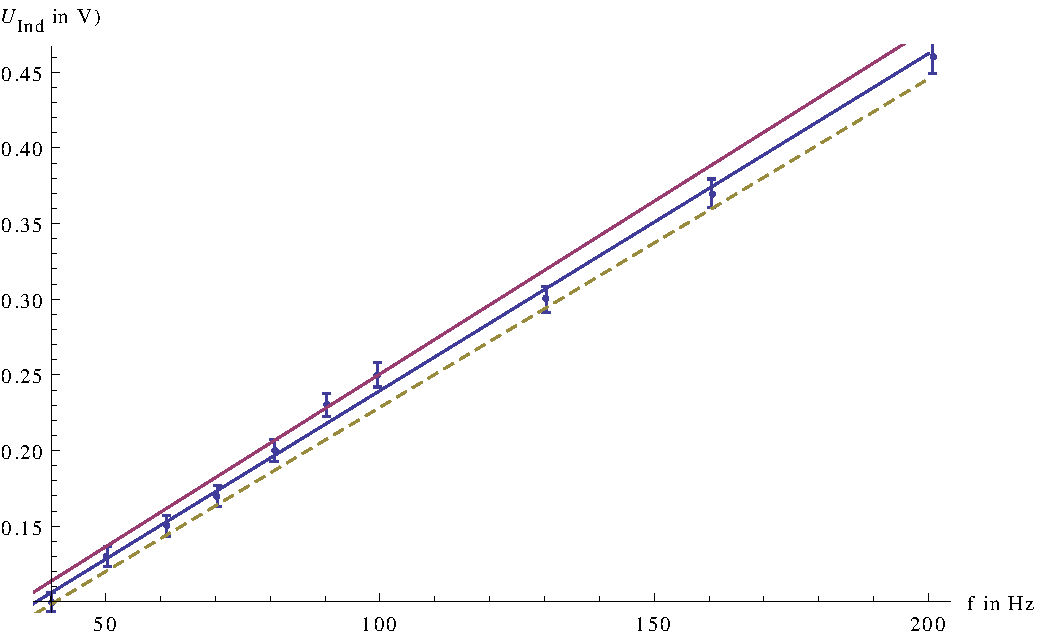
\includegraphics[width=11cm]{graph3}
	Induktionsspannungsverlauf in Abhängigkeit vom Anstellwinkel \( \alpha \)
\end{center}

Die Steigung \(b\) und der Ordinatenabschnitte \(a\) wurde mittels linearer Regression bestimmt zu

\begin{center}
\begin{tabular}{c c c c c} 
  \(b\) & = & \(0,002228\) & \(\pm \) & \(0,000057 \) \\ 
  \(a\) & = & \(0,0168\) & \(\pm \) & \(0,0053 \) \\ 

 \end{tabular}
\end{center}

\subsection{Auswertung}
Der Stromverlauf in der Feldspule kann beschrieben werden durch
\begin{equation}
I(t) = I_0 \sin(\omega t + \varphi_0)
\notag
\end{equation}
Gemessen wurde allerdings \( I_{eff} = (8,75 \pm 0,10)\,mA \). Es gilt jedoch nach \eqref{U_eff} für \( U_{eff} \) analog für
\begin{equation}
I_{eff} = \frac{I_0}{\sqrt{2}}
\notag
\end{equation}
somit folgt
\begin{equation}
I(t) = I_{eff} \cdot \sqrt{2} \cdot \sin(\omega t + \varphi_0)
\label{I_sinus}
\end{equation}
Wie In \eqref{U_induktionsspule} und \eqref{B_induktionsspule} gilt wieder
\begin{equation}
U_{ind} = -N \cdot A \cdot \frac{\partial B}{\partial t}
\notag
\end{equation}

\begin{equation}
B(t) = \frac{L_{Feld}}{n_{Feld} \cdot A_{Feld}} \cdot I(t)
\notag
\end{equation}
Mit \eqref{I_sinus} folgt
\begin{equation}
U(t) = -\frac{n_{Ind} \cdot A_{Ind}}{n_{Feld} \cdot A_{Feld}} \cdot L_{Feld} \cdot I_{eff} \cdot \sqrt{2} \cdot \omega \cdot \cos(\omega t + \varphi_0)
\notag
\end{equation}
und mit \eqref{U_eff}
\begin{equation}
U_{eff}(f) = \frac{n_{Ind} \cdot A_{Ind}}{n_{Feld} \cdot A_{Feld}} \cdot L_{Feld} \cdot I_{eff} \cdot 2\pi \cdot f
\label{U_eff(t)}
\end{equation}
Qualitativ stimmt das Ergebnis also mit der Beobachtung eines linearen verlaufs überein. Außerdem können wir die Steigung \(b\) identifizieren als
\begin{align}
b &= \frac{n_{Ind} \cdot A_{Ind}}{n_{Feld} \cdot A_{Feld}} \cdot L_{Feld} \cdot I_{eff} \cdot 2\pi
= 0,0002420 \,Vs
\notag
\\
\Delta b &= b \cdot \sqrt{
\left( \frac{\Delta A_{Ind}}{A_{Ind}} \right)^2 +
\left( \frac{\Delta A_{Feld}}{A_{Feld}} \right)^2 +
\left( \frac{\Delta L_{Feld}}{L_{Feld}} \right)^2 +
\left( \frac{\Delta I_{eff}}{I_{eff}} \right)^2
}
\notag
\\
&= 0,0000029 \, Vs
\notag
\end{align} 
\subsection{Fazit}
Es wurde folgendes Ergebnis für die Steigung \(b\) ermittelt
\begin{center}
\begin{tabular}{c c} 
 Messwert & Angabe/Theorie \\
 \( (2,23 \pm 0,06)\, mVs \) & \( (0,242 \pm 0,003)\, mVs \) \\
 \end{tabular}
\end{center}
Damit sind die Werte signifikant unterschiedlich. Sie sind sogar völlig verschieden. Es ist zu vermuten, dass eine Messgröße falsch aufgenommen wurde oder ein schwererwiegender systematischer Fehler aufgetreten ist. Da die Werte etwa um den Faktor \(10\) verschieden sind, ist es auch möglich, dass eine Messskala falsch notiert wurde. Die theoretische Herlitung konnte somit jedoch nicht bestetigt werden. Das die theoretische Betrachtung einen Fehler enthält soll jedoch nicht ausgeschlossen werden. Am rande sei noch erwähnt, dass der Ordinatenabschnitt mit dreifachem Fehlerintervall den Nullpunkt umschließt. es kann sich also prinzipiell um eine Ursprungsgerade handeln.

\section{Aufgabe 3}
\subsection{Aufbau}
Ähnlich wie in Aufgabe 2 wurde die Feldspule über ein Multimeter (FLUKE True RMS 175), zur Strommessung, mit dem Funktionsgenerator verbunden. Anschließend wurde eine drehbare kleine Spule mit messbarem Winkel \( \alpha \) in die Feldspule gebracht. Gemessen wurde die Induktionsspannung an der drehbaren Spule \( U_{Ind} \) (Voltcraft VC 220).
\subsection{Fehlerabschätzung}
Da wir den Winkel \( \alpha \) mit einem Geodreieck selbst einstellen konnten ist diese Messgröße nur wenig Fehlerbehaftet. Der Strom war über die ganze Zeit sehr konstant und konnte sehr genau gemessen werden. Es wird also der Fehler der Spannung \( \Delta U_{Ind} = (1,2\% \, + \, 5d ) \) herangezogen.
\subsection{Gegebenes}
\begin{center}
\begin{tabular}{c c c}
 & Feldspule & Induktionsspule \\
 \(N\) & \(1000\) & \(300\) \\
 \(A\) & \((19,73 \pm 0,02)\, cm^2\) & \((4,15 \pm 0,18)\, cm^2\) \\
 \(L\) & \((10,89 \pm 0,03)\, mH \) & nicht benötigt \\
 \(l\) & \((0,190 \pm 0,001)\, m\ \) & \((0,0070 \pm 0,0002)\, m\ \) \\
\end{tabular}
\end{center}
\subsection{Beobachtung}
Es war zu sehen, dass die induzierte Spannung mit größer werdenden \( \alpha \) abnahm. In welcher Form war nicht sofort ersichtlich. Die Änderung des Stroms wurde aber mit größerem \( \alpha \) auch größer. 
\subsection{Messwerte und Graph}

\begin{center}


\begin{tabular}{l l l l l}
\(\alpha\)[\(\circ\)] & cos(\(\alpha\))[rad] & \(U_{Ind}[mV]\) & \(\Delta U_{Ind}[mV]\) \\
\(0\) &	\(1.00\) &	\(53.5\) &	\(1.0\) \\
\(10\) &	\(0.99\) &	\(52.7\) &	\(1.0\)\\
\(20\) &	\(0.94\) &	\(50.5\) &	\(1.0\)\\
\(30\) &	\(0.87\) &	\(46.9\) &	\(1.0\)\\
\(40\) &	\(0.77\) &	\(41.8\) &	\(0.9\)\\
\(50\) &	\(0.65\) &	\(35.8\) &	\(0.9\)\\
\(60\) &	\(0.50\) &	\(25.8\) &	\(0.8\)\\
\(70\) &	\(0.35\) &	\(17.2\) &	\(0.7\)\\
\(80\) &	\(0.18\) &	\(9.3\) &	\(0.6\)\\
\(90\) &	\(0.00\) &	\(0.6\) &	\(0.5\)\\
\end{tabular}\\
Messung der Spannung in Abhängigkeit vom Winkel \(\alpha\)\\
\end{center}
Der Strom war sehr kosntant \(I_{Feld} = (127,9 \pm 0,1)\, mA\).

\begin{center}
  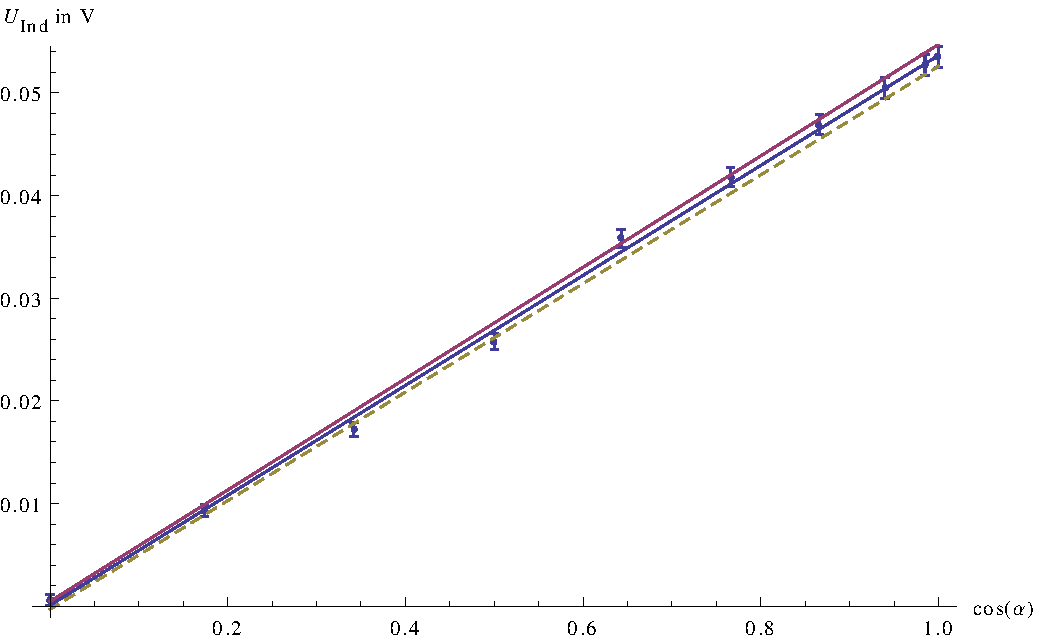
\includegraphics[width=11cm]{graph4}
	Induktionsspannungsverlauf in Abhängigkeit vom Anstellwinkel \( \alpha \)
\end{center}
Die Steigung \(b\) und der Ordinatenabschnitte \(a\) wurde mittels linearer Regression bestimmt zu

\begin{center}
\begin{tabular}{c c c c c} 
  \(b\) & = & \(0,05358\) & \(\pm \) & \(0,00068 \) \\ 
  \(a\) & = & \(0,000081\) & \(\pm \) & \(0,00038 \) \\ 

 \end{tabular}
\end{center}

\subsection{Auswertung}
Der einzige Unterschied zur Relation in \eqref{U_eff(t)} ist, dass \(\vec{B} \cdot \vec{A} = A \cdot B \cdot \cos(\alpha) \) und nicht mehr \(\vec{B} \cdot \vec{A} = A \cdot B \). Deshalb gilt
\begin{equation}
U_{eff}(\alpha) = \frac{n_{Ind} \cdot A_{Ind}}{n_{Feld} \cdot A_{Feld}} \cdot L_{Feld} \cdot I_{eff} \cdot 2\pi \cdot f \cdot \cos(\alpha)
\notag
\end{equation}
Qualitativ stimmt das Ergebnis also mit der Beobachtung eines linearen verlaufs von \( U_{Ind} \) zu \( \cos(\alpha) \) überein. Außerdem können wir die Steigung \(b\) identifizieren als
\begin{align}
b &= \frac{n_{Ind} \cdot A_{Ind}}{n_{Feld} \cdot A_{Feld}} \cdot L_{Feld} \cdot I_{eff} \cdot 2\pi \cdot f
= 0,0558 \,V
\notag
\\
\Delta b &= b \cdot \sqrt{
\left( \frac{\Delta A_{Ind}}{A_{Ind}} \right)^2 +
\left( \frac{\Delta A_{Feld}}{A_{Feld}} \right)^2 +
\left( \frac{\Delta L_{Feld}}{L_{Feld}} \right)^2 +
\left( \frac{\Delta I_{eff}}{I_{eff}} \right)^2
}
\notag
\\
&= 0,0024 \, V
\notag
\end{align}

\subsection{Fazit}
Es wurde folgendes Ergebnis für die Steigung \(b\) ermittelt
\begin{center}
\begin{tabular}{c c} 
 Messwert & Angabe/Theorie \\
 \( (53,6 \pm 0,7)\, mV \) & \( (56 \pm 3)\, mV \) \\
 \end{tabular}
\end{center}
Somit sind die Ergebnisse gleich. Wir können die theoretische Abhängigkeit der Induktionsspannung vom Winkel der Induktionsspule zum Magnetfeld bestätigen. Das Fehlerintervall des Ordinatenabschnitts umschließt den Nullpunkt, daher kann es sich auch um eine Ursprungsgerade handeln.

\newpage
\section{zu den ergänzenden Fragen}
Wie hängen die Induktionsspannung von der Frequenz ab, wenn an der Feldspule nicht der Strom, sondern die Spannung konstant gehalten wird?
Beobachten Sie auf dem Oszilloskop die Phasenlage zwischen Feld- und Induktionsspannung in Abhängigkeit von der Frequenz.
Begründen Sie, warum bei genügend hoher Frequenz die Spannung phasengleich sind. Belasten Sie die Induktionsspule zusätzlich (niederohmig). Warum tritt jetzt auch bei hohen Frequenzen eine Phasenverschiebung auf (Energiebetrachtung).

\vspace{1cm}

Da es nach dem Einschaltvorgang einer Gleichspannnung keine Stromänderung in der Feldspule mehr gibt, gibt es auch keine Magnetfeldänderung. Das hat zur Folge, dass keine Spannung in die Induktionsspule induziert wird. Wenn man allerdings bei einer Wechselspannung den Effektivwert konstant hält, kann man währenddessen die Abhängigkeit von der Induktionsspannung und der Frequenz beobachtet.
Da sich eine Spule in einem Wechselstromkreis durch die Impedanz $Z=\omega L$ beschreiben lässt, kommt man mit dem Effektivwert auf das Ohm'sche Gesetz:

\begin{equation}
U_{eff}=\omega L I_{eff}=2\pi L I_{eff}
\notag
\end{equation}

Soll die Spannung konstant bleiben, muss im Umkehrschluss bei einer Erhöhung der Frequenz der Effektivwert des Stroms kleiner werden. Dies hat widerum zur Folge, dass die Induktionsspannung abnimmt, da sie proportional zum Strom ist.

Die Gesetze der Wechselstromkreise besagen, dass eine Spule eine Phasenverschiebung von $\dfrac{\pi}{2}$ zwischen Spannung und Strom verursacht. Da sich nun unser Magnetfeld in Phase mit dem Stron ändert, ändert sich auch die Induktionsspannung in Phase mit dem Strom. Daraus folgt, dass der Phasenunterschied zwischen Feld- und Induktionsspannung $\dfrac{\pi}{2}$ beträgt.\\

Wenn wir jetzt in den kHz- bzw MHz-Bereich gehen, treten Resonanzphänomene auf. Diese Phänomene verursachen eine weitere Phasenverschiebung, da sich das System nun wie ein R-C-L-Kreis verhält. Um nun aus der Blindleistung im Primärkreislauf eine Verlustleistung wird, die wir benötigen damit Energie in den Sekundärkreislauf kommt, muss Strom mithilfe eines Lastwiderstands an der Induktionsspule fließen. Da aber am Lastwiderstand Energie verloren gehen wird, muss ein Teil des Stroms in Phase mit der Spannung sein, wodurch auch bei hohen Frequenzen eine Phasenverschiebung zwischen Feld- und Induktionsspannung folgt.\\

\newpage

\section{Fazit}

Die Versuche waren alle sehr gut durchführbar und es gab keine großen Probleme Messgrößen zu ermitteln. Die Ergebnisse der Messung (mit Ausnahme der Steigung in A2) stimmen sehr gut mit den theoretischen Vorhersagen überein. Schwierig war es hingegen die genaue Aufgabenstellung herauszufinden, da das Skript dazu etwas unpräzise ist. 

\section{Quellen}
\begin{itemize}
\item Das GP2-Skript der FU-Berlin
\item Das Theoretische Physik 4 Skript von Tamara Nunner (FU-Berlin)
\end{itemize}

\end{document}